\documentclass[12pt, a4paper]{article}

\usepackage{graphicx}


\title{Notulensi Pertemuan}
\author{BMKG 2}
\date{9 July 2022}

\begin{document}
\maketitle

\begin{tabbing}
\textbf{Hari/Tanggal}\quad\= Sabtu, 9 July 2022 \\
\textbf{Waktu} \>13.00 - 15.30 \\
\textbf{Tempat}\> Zoom Meeting
\end{tabbing}

Agenda pertemuan hari ini adalah:
\begin{enumerate}
\item eksplorasi dataset,
\item evaluasi dataset,
\item pembahasan mekanisme \emph{demo day},
\item pembagian tugas individu
\end{enumerate}

\bigskip 
Pada pertemuan kedua kami mendiskusikan tentang parameter input dan target yang sudah kami tentukan sebelumnya. Hasil dari diskusi tersebut adalah kami menambahkan \textbf{``cloud"} sebagai parameter input karena mempunyai data yang lengkap dan sangat potensial sebagai penentu apakah di jam tersebut terjadi hujan atau tidak. Selain menambahkan parameter input kami juga menambahkan \textbf{``rain\_1h"} sebagai target.

\medskip
Setelah disepakati bersama tentang parameter input dan target, kami menentukan model \emph{machine learning} apa yang sesuai dengan data BMKG yang telah disediakan oleh instruktur. Berdasarkan hasil diskusi kami akan menggunakan dua pendekatan berbeda untuk mengolah dataset yang telah diberikan. Pertama kami akan menggunakan model \emph{machine learning} dengan teknik \emph{time series} dan model lainnya adalah dengan menggunakan teknik \emph{supervised learning}. Kedua model itu akan menggunakan parameter input dan target yang berbeda. Hasil prediksi dari kedua model tersebut nantinya akan kami evaluasi lebih lanjut untuk melihat seberapa banyak perbedaan yang dihasilkan diantara keduanya.

\medskip
Selanjutnya, pada pertemuan hari ini kami membagi tugas berdasarkan elemen yang ada pada mekanisme \emph{demo day}. Seperti yang diketahui bersama elemen dari \emph{demo day} adalah sebagai berikut:
\begin{enumerate}
\item \emph{coding},
\item proposal,
\item presentasi,
\item laporan akhir dan dokumentasi,
\end{enumerate}
Setelah berdiskusi akhirnya kami membagi tugas per individu sesuai dengan elemen \emph{demo day} dan tambahan dua orang untuk \emph{coding}, untuk jelasnya dapat dilihat pada gambar \ref{fig:pert-21}. Pada pertemuan hari ini kami juga membahas tentang rencana pengerjaan dari setiap elemen \emph{demo day} seperti yang ada pada gambar \ref{fig:pert-22}.


\bigskip
\section*{Dokumentasi}
\begin{figure}[h]
    \centering
    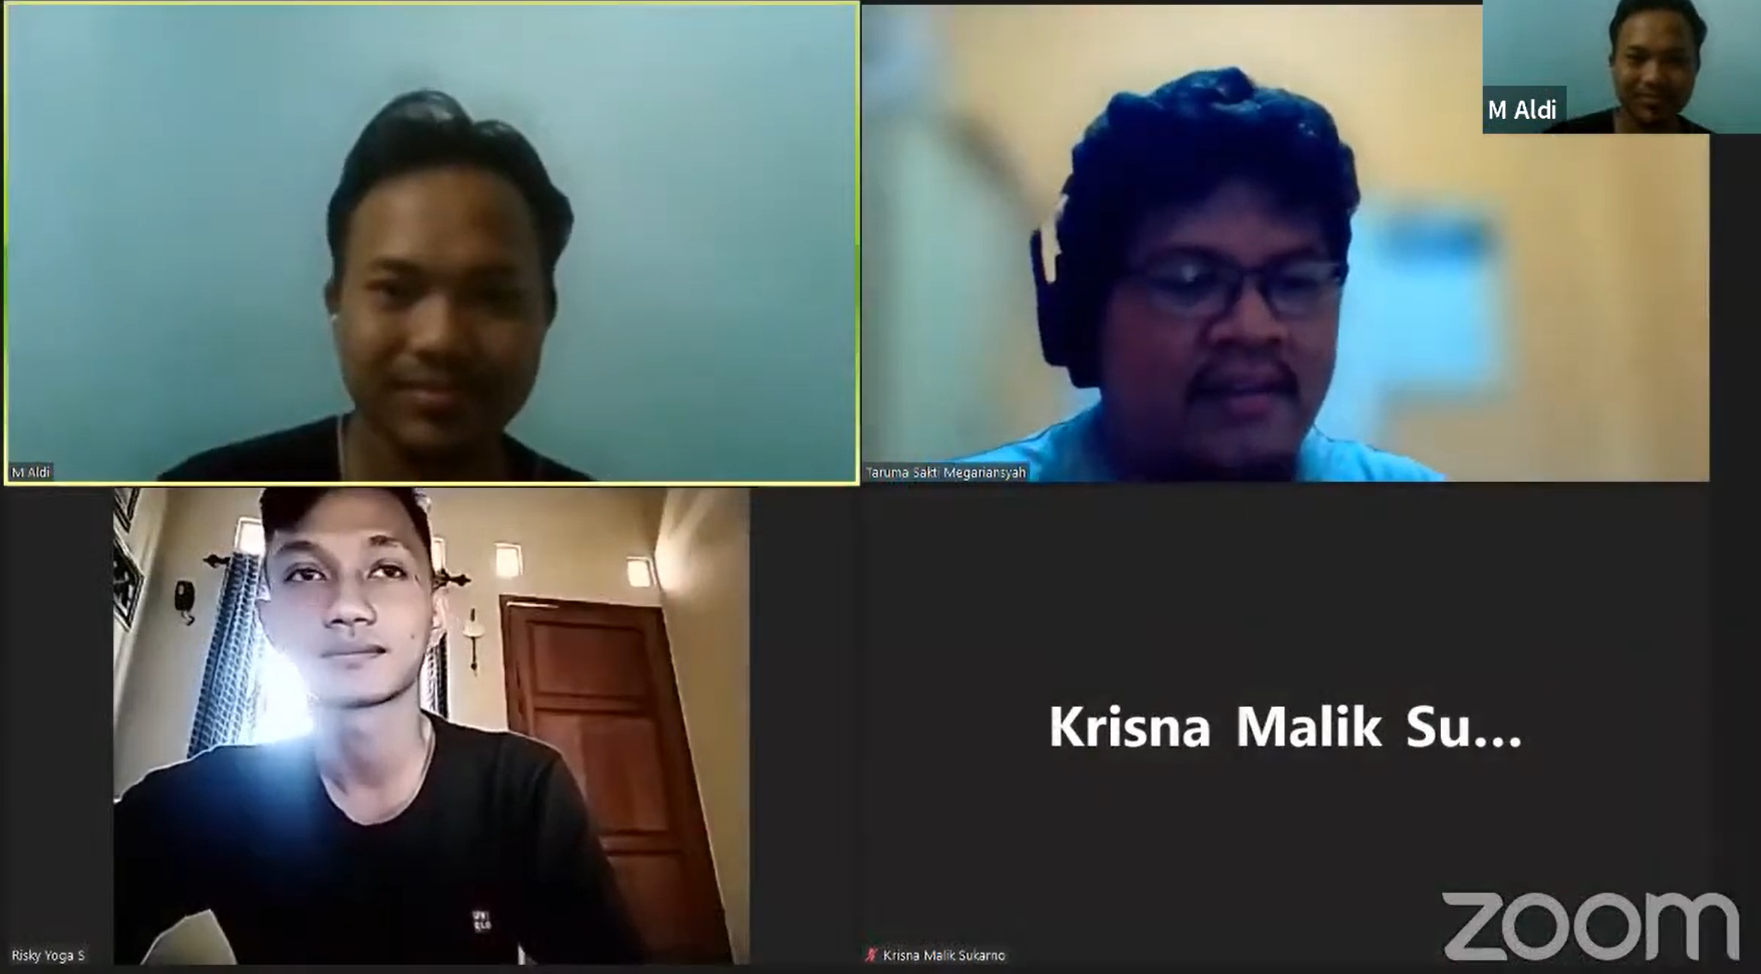
\includegraphics[width=\textwidth]{pert-2}
    \caption{Pertemuan Kedua}
\end{figure}

\begin{figure}[h]
    \centering
    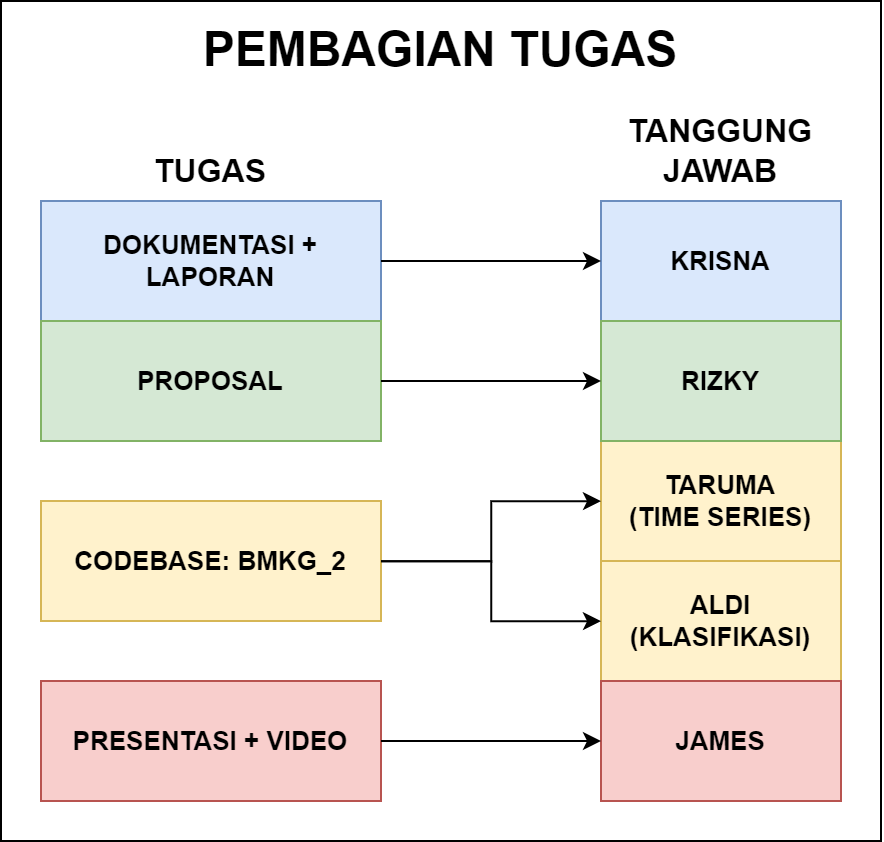
\includegraphics[width=\textwidth]{pert-21}
    \caption{Pembagian Tugas}
    \label{fig:pert-21}
\end{figure}

\begin{figure}[h]
    \centering
    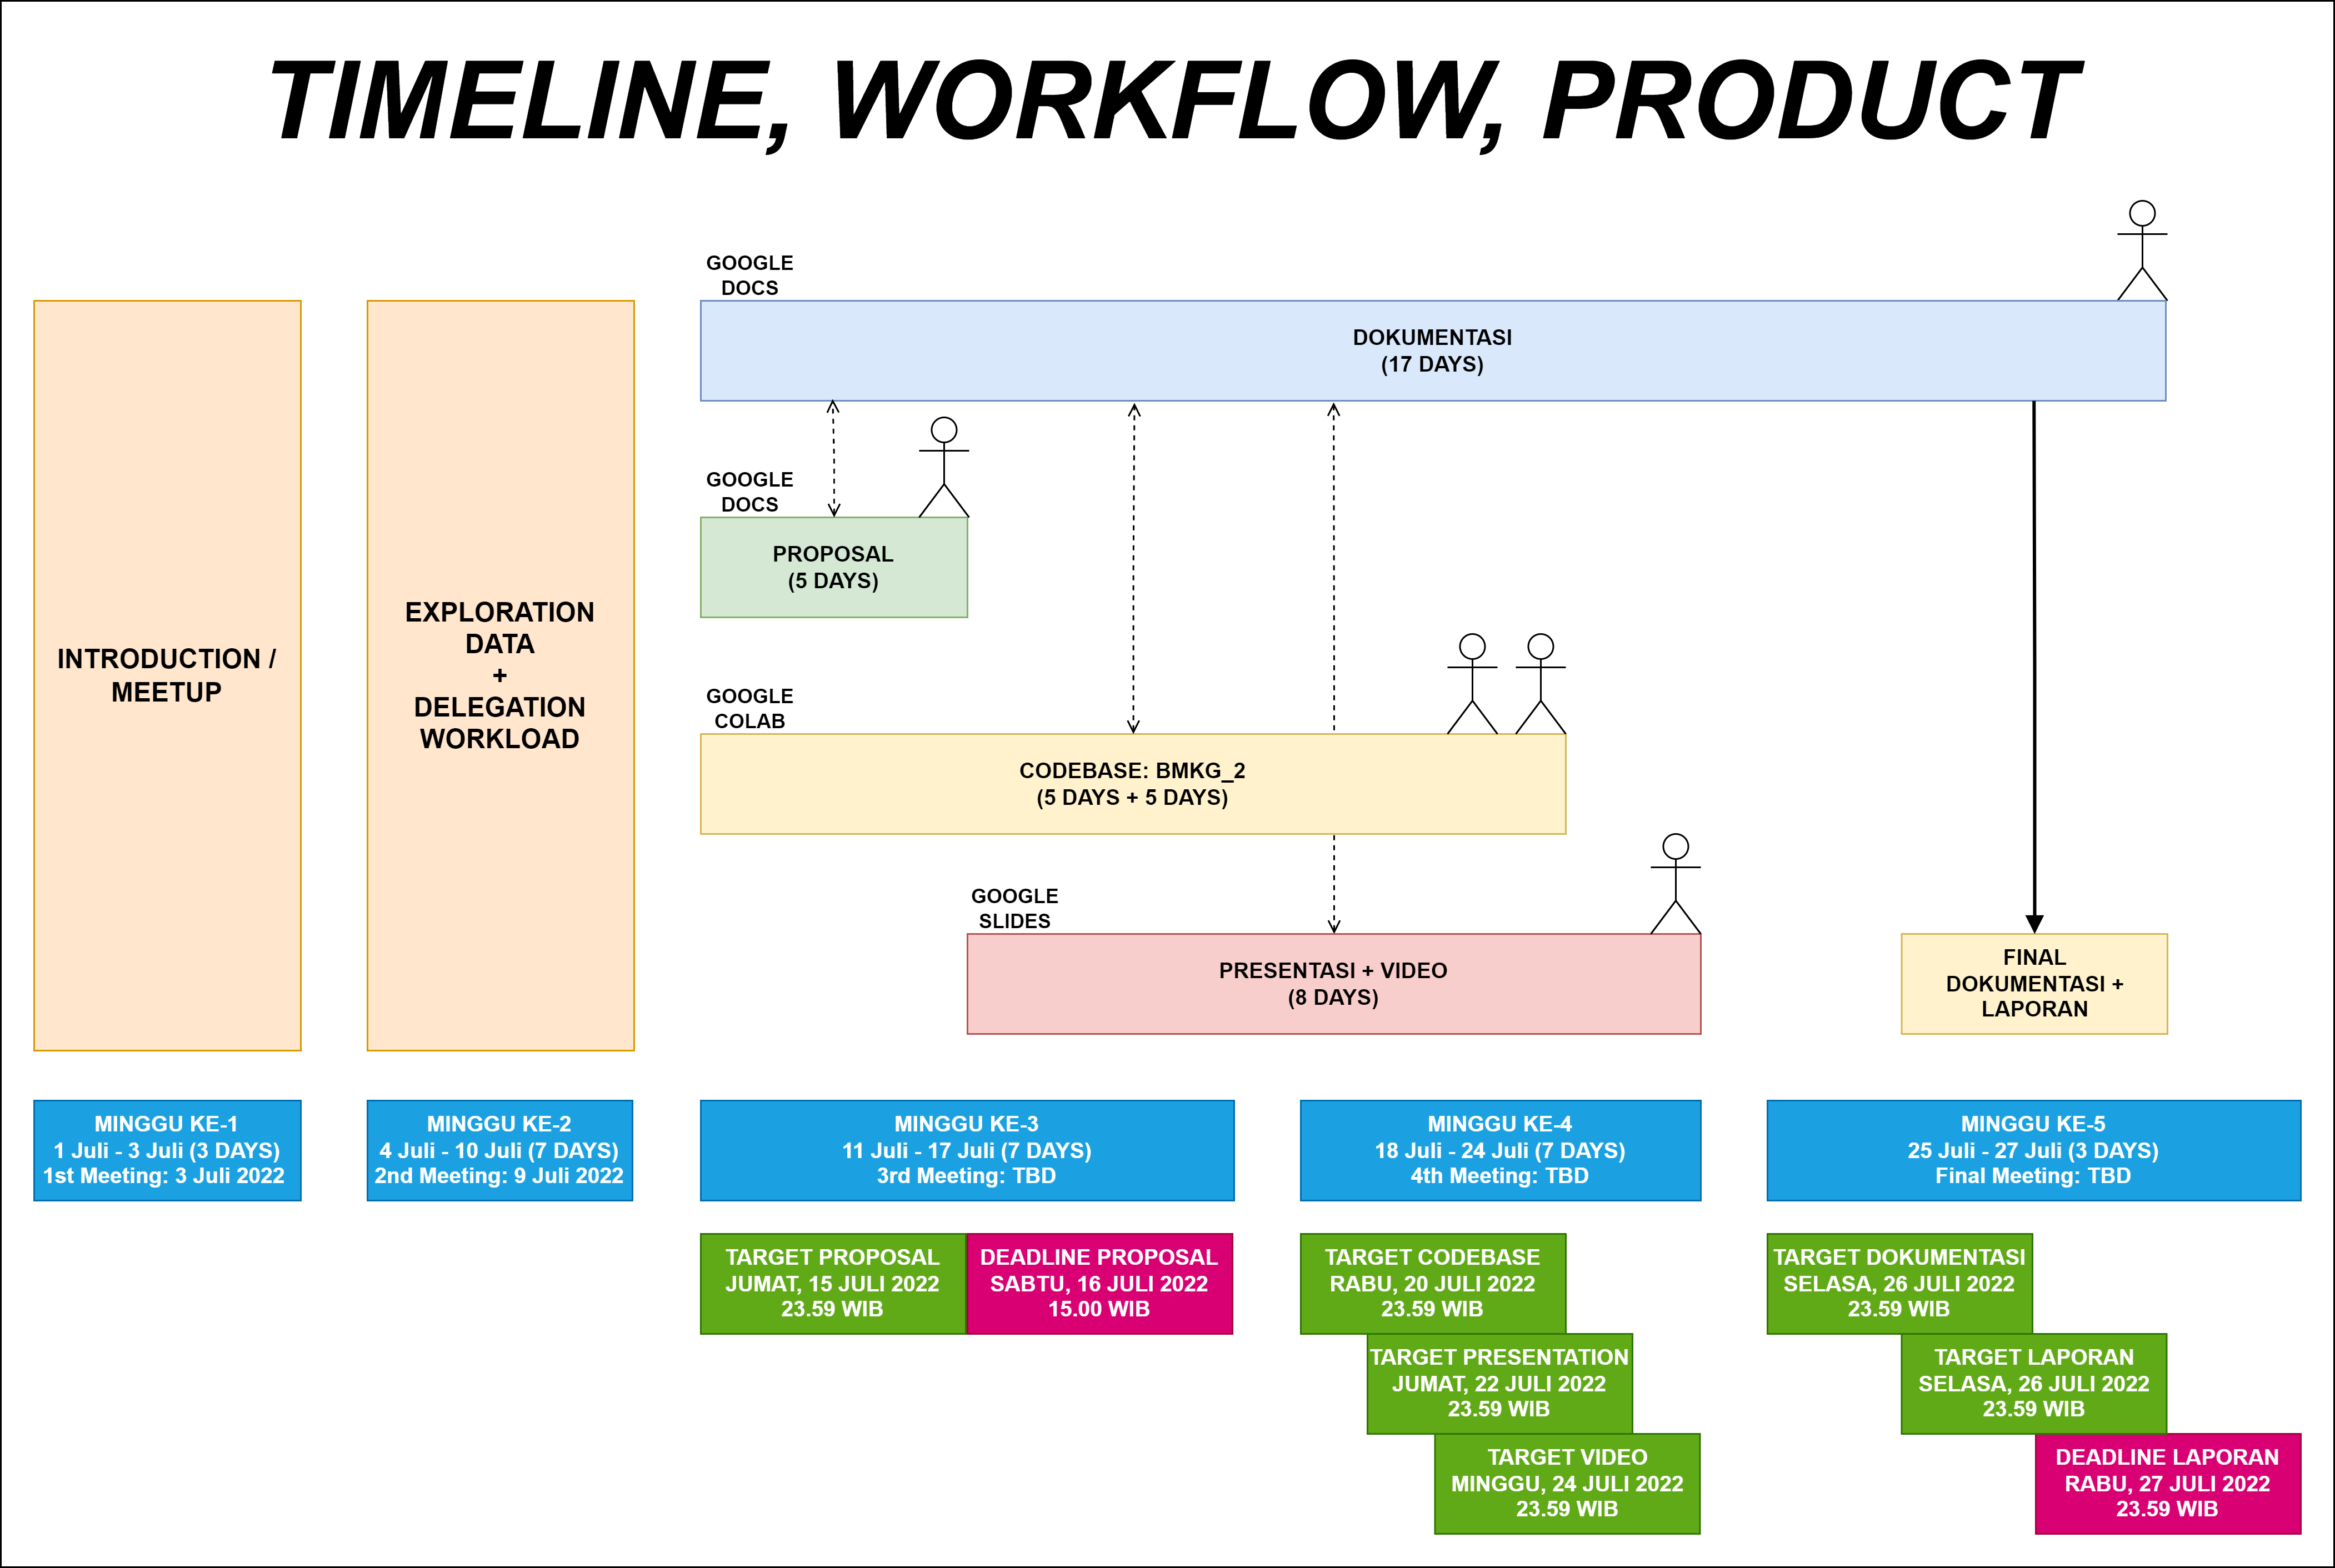
\includegraphics[width=\textwidth]{pert-22}
    \caption{Rencana Pengerjaan}
    \label{fig:pert-22}
\end{figure}

\end{document}